\chapter{The projective plane}\label{chapter:projective.plane}
\epigraph[author={Arthur Cayley}]{The more systematic course in the present introductory memoir \dots
would have been to ignore altogether the notions of distance and
metrical geometry \dots. Metrical geometry is a part of descriptive
geometry, and descriptive geometry is all geometry.}\SubIndex{Cayley, Arthur}
The old fashioned term \emph{descriptive geometry}\define{descriptive geometry} means the geometry of straight lines.
Straight lines in the plane remain straight when you rescale the plane, or translate the plane to the left or right, up or down, or when you rotate the plane.
They even remain straight when you carry out any linear change of variables, as you know from linear algebra.

\bigskip

\epigraph[author={William Blake}, source={Auguries of Innocence}]{To see a World in a Grain of Sand, \\ And Heaven in a Wild Flower. \\ Hold Infinity in the palm of your hand, \\ And Eternity in an hour.}\SubIndex{Blake, William}

Railway tracks built on a flat plane appear to meet ``at infinity''.
\begin{center}
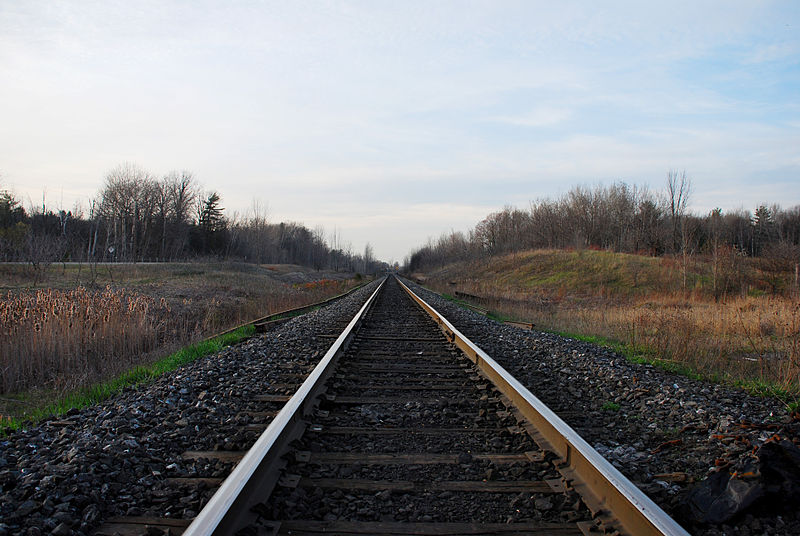
\includegraphics[width=4cm]{railway-tracks.jpg} \\[2pt]
\begin{minipage}{4cm}\raggedright\tiny{Creative Commons Attribution-Share Alike 3.0 Unported license. I, MarcusObal}\end{minipage}
\end{center}
Imagine that we were to add a point to the plane ``at infinity'' in the direction where these tracks (straight lines) appear to meet.
\emph{Danger:} in order to add only one point, imagine that the two rails meet at the \emph{same} point in one direction as they do in the other, making them both into circles.
The projective plane is the set of all of the usual points of the plane (which we can think of as the ``finite points'' of the projective plane) together with some sort of ``points at infinity'' to represent the directions in the plane.

\epigraph[author={Fyodor Dostoyevsky}, source={The Brothers Karamazov}]{
But you must note this: if God exists and if He really did
create the world, then, as we all know, He created it according to
the geometry of Euclid and the human mind with the conception
of only three dimensions in space.  Yet there have been and
still are geometricians and philosophers, and even some of the
most distinguished, who doubt whether the whole universe, or
to speak more widely the whole of being, was only created in
Euclid's geometry; they even dare to dream that two parallel
lines, which according to Euclid can never meet on earth, may
meet somewhere in infinity.}\SubIndex{Dostoyevsky, Fyodor}\SubIndex{Brothers Karamazov}


We would like a more precise mathematical definition of points ``at infinity''.
A \emph{pencil}\define{pencil} of parallel lines is the collection of all lines parallel to a given line:
\[
\begin{tikzpicture}
\clip (0,0) rectangle (1,1);
\foreach \i in {-1,-0.9,...,1} 
{
	\draw (0,{\i}) -- (1,{\i+1});
}
\end{tikzpicture}
\]
A simple approach: just say that a ``point at infinity'' means nothing more than a choice of pencil of parallel lines.

There is another completely different way to give a precise mathematical definition of the projective plane, which is more geometric and more powerful.
Place yourself at a vantage point above the plane.
\begin{center}
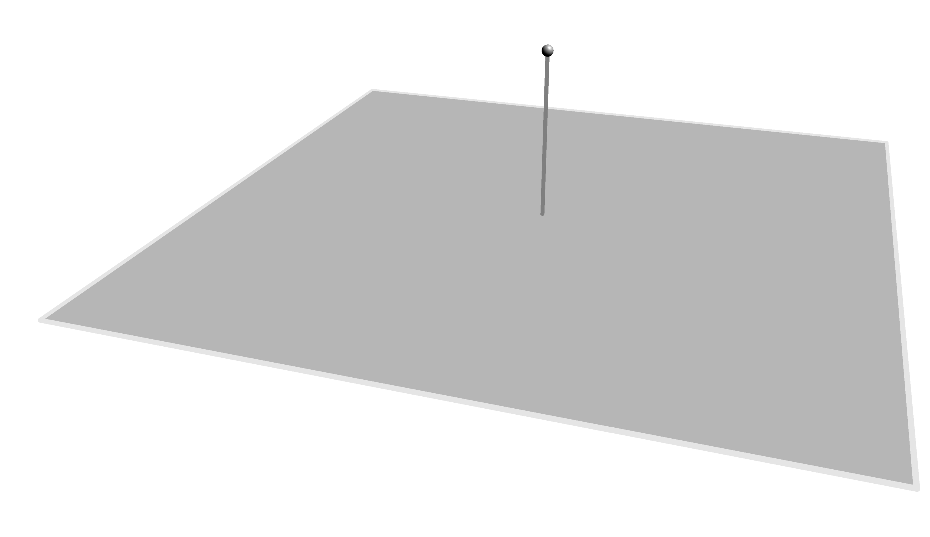
\includegraphics[width=4cm]{above-the-plane-vantage}
\end{center}
Every ``finite'' point of the plane lies on a line through your vantage point: the line of sight.
\begin{center}
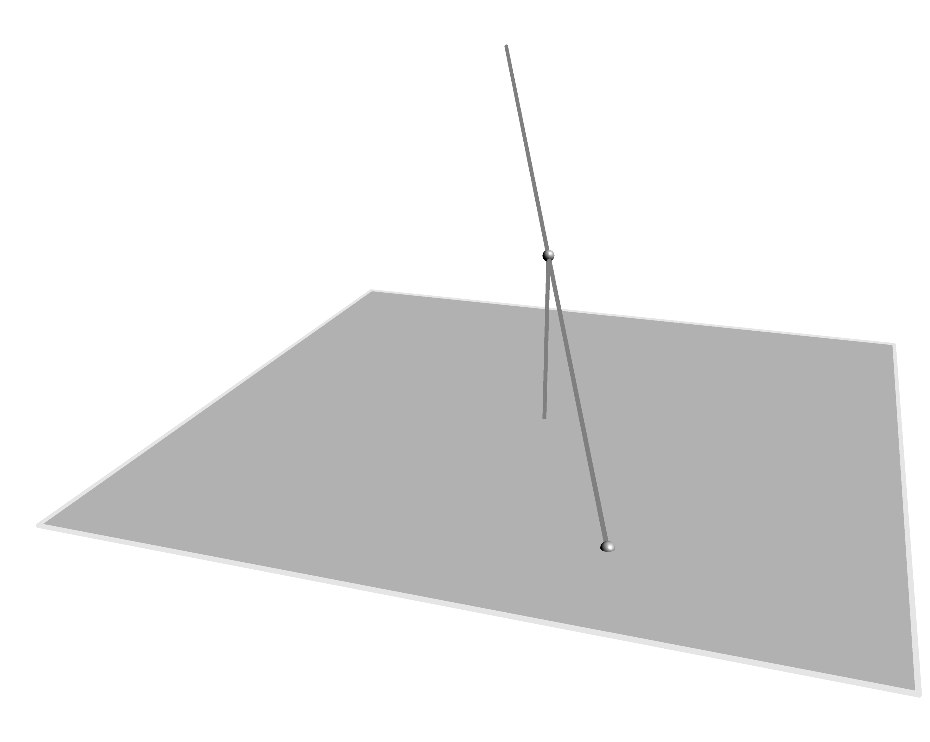
\includegraphics[width=4cm]{above-the-plane-connect}
\end{center}
You can also look out to the points at infinity, along lines:
\begin{center}
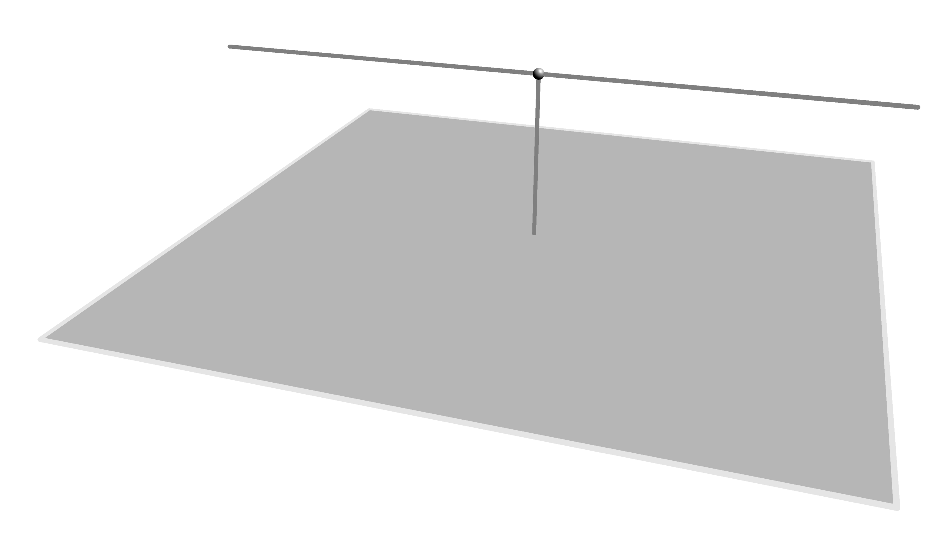
\includegraphics[width=4cm]{above-the-plane-off-to-infinity}
\end{center}
For example, there is such a line  parallel to the lines of our train track:
\begin{center}
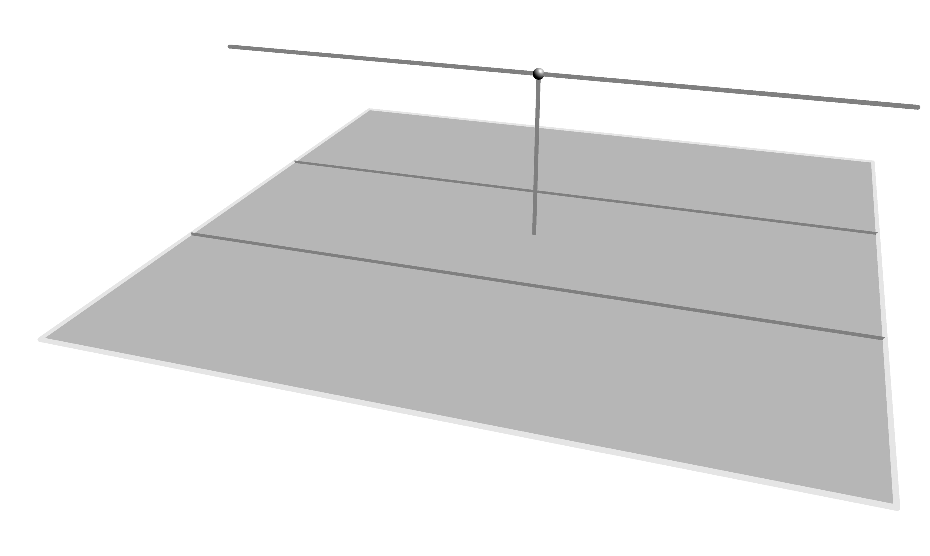
\includegraphics[width=4cm]{above-the-plane-3}
\end{center}

On the other hand, if we take any line through the vantage point, either it hits a ``finite'' point of the plane:
\begin{center}
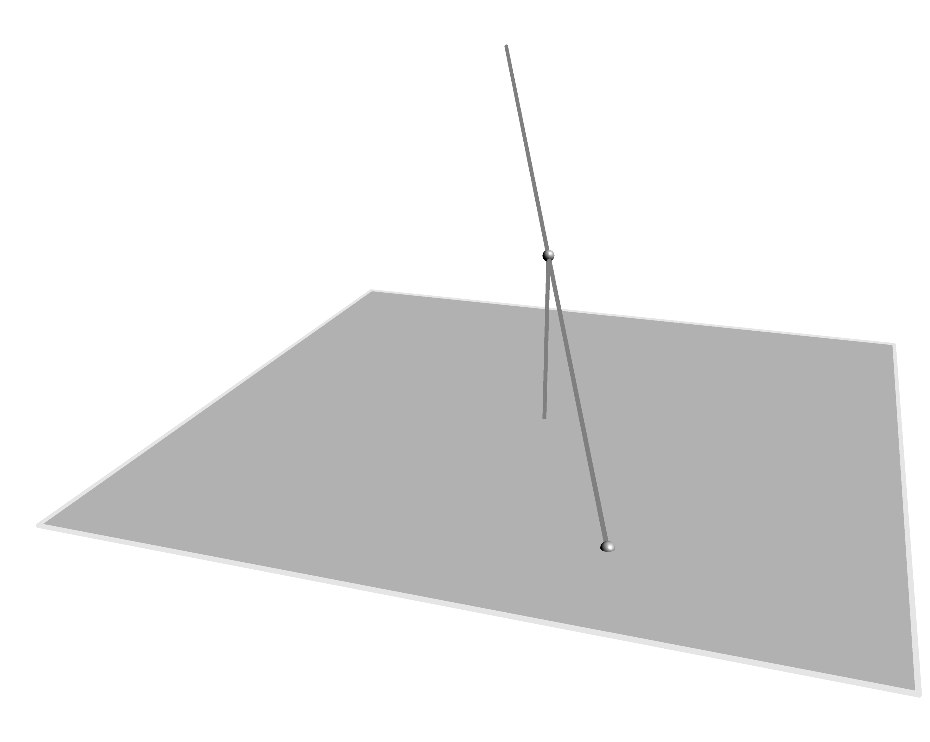
\includegraphics[width=4cm]{above-the-plane-connect}
\end{center}
or it is parallel to the plane
\begin{center}
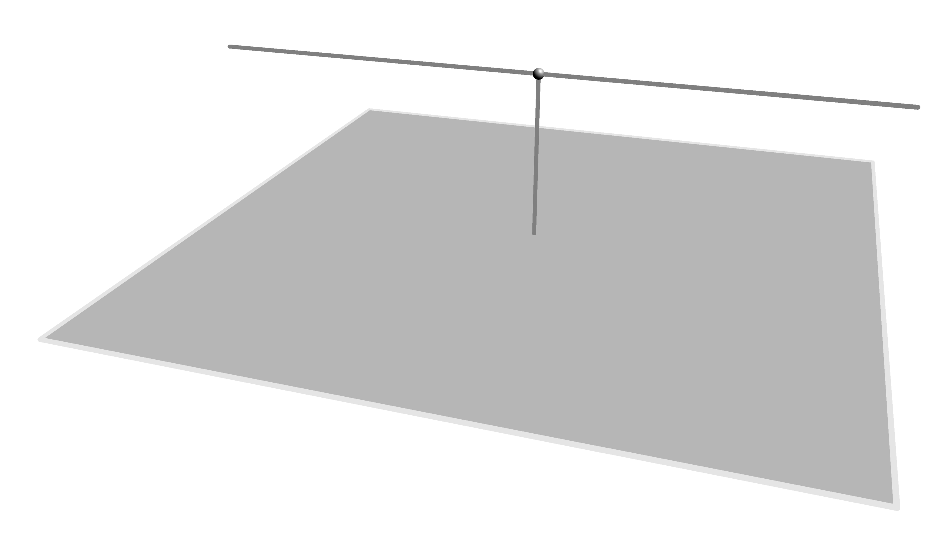
\includegraphics[width=4cm]{above-the-plane-off-to-infinity}
\end{center}
so that it is pointed along the direction of some train tracks (lines) in the plane, to some ``point at infinity''.
\begin{center}
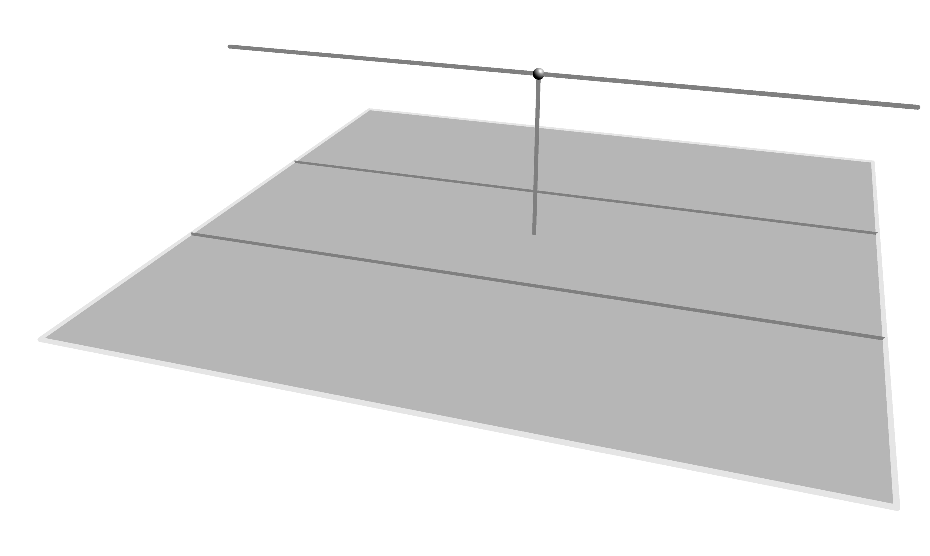
\includegraphics[width=4cm]{above-the-plane-3}
\end{center}
The points of the projective plane, finite points together with infinite points at infinity, are in 1-1 correspondence with lines through the vantage point.

This picture gives us a rigorous definition of points at infinity: the \emph{projective plane}\define{projective!plane} is the set of all lines through a chosen point of 3-dimensional space, called the vantage point.
The \emph{points} of the projective plane (using this definition) are the lines through the vantage point.
The ``finite points'' are the lines not parallel to the horizontal plane, while the ``infinite points'' are the lines which are parallel the horizontal plane.
The \emph{lines}\define{projective!line}, also called \emph{projective lines}, of the projective plane are the planes through the vantage point.




\section{Homogeneous coordinates}
We can make this more explicit by writing each point of 3-dimensional space \(\R{3}\) as a triple \((x,y,z)\).
Draw the plane not as the usual \(xy\)-plane, but as the plane \(z=z_0\), for some nonzero constant \(z_0\).
Take the vantage point to be the origin.
Any linear change of the 3 variables \(x,y,z\) takes lines (and planes) through the origin to one another: there are more symmetries of the projective plane than we encountered before.

Every point of 3-dimensional space not at the origin lies on a unique line through the origin.
So every point \((x,y,z)\) with not all of \(x,y,z\) zero lines on a unique line through the origin.
The points of this line are precisely the rescalings \((tx,ty,tz)\) of that point.
So each point of the projective plane can be written as a triple \((x,y,z)\), not all zero, and two such triples represent the same point just when each is a rescaling of the other.
Denote such a point as \([x,y,z]\).
For example, the point \([3,1,2]\) of the projective plane means the line through the origin consisting of the points of the form \((3t,t,2t)\) for all values of a variable \(t\), including \((3,1,2)\), \((3 \cdot 2, 1 \cdot 2, 2 \cdot 2)\), \((-3,-1,-2)\), and so on.
We write this as:
\[
[3,1,2]=[3 \cdot 2, 1 \cdot 2, 2 \cdot 2]=[-3,-1,-2].
\]
The coordinates \(x,y,z\) are the \emph{homogeneous coordinates}\define{homogeneous!coordinates}\define{coordinates!homogeneous} of a point \([x,y,z]\) of the projective plane.

In our pictures, the plane \(z=z_0\) was below the vantage point, but it is more traditional to take the plane to be \(z=1\), above the vantage point.
The \emph{affine plane} is just the usual \(xy\) plane, but identified either with the plane \(z=1\), or with the subset of the projective plane given by points \([x,y,1]\).

The roles of \(x,y,z\) are all the same now, and we can see that any linear change of variables of \(x,y,z\) takes the points of the projective plane to one another, and takes the lines of the projective plane to one another.
Each linear change of variables is represented by an invertible matrix
\[
g=
\begin{pmatrix}
g_{00} & g_{01} & g_{02} \\
g_{10} & g_{11} & g_{12} \\
g_{20} & g_{21} & g_{22}
\end{pmatrix}.
\]
Conventionally we label our matrix columns using \(0,1,2\) rather than \(1,2,3\).
Such a matrix takes a point \(p=[x,y,z]\) of the plane to the point \(q=[X,Y,Z]\) where
\[
\begin{pmatrix}
X \\
Y \\
Z
\end{pmatrix}
=
g
\begin{pmatrix}
x \\
y \\
z
\end{pmatrix}.
\]
We denote this relation as \(q=[g]p\) and call \([g]\) a \emph{projective automorphism}\define{projective!automorphism}.
Clearly if \(g\) and \(h\) are 2 invertible \(3 \times 3\) matrices, then \([gh]=[g][h]\), i.e. we carry out the transformation of lines through the origin by carrying out the multiplications by the matrices.

\begin{lemma}
If a square matrix \(g\) rescales every nonzero vector by a scalar, i.e. \(gx=\lambda(x)x\) for some number \(\lambda(x)\), for every vector \(x \ne 0\), then \(\lambda(x)\) is a constant scalar independent of \(x\).
\end{lemma}
\begin{proof}
Suppose that \(g\) is \(n \times n\).
If \(n=1\) then every square matrix is a constant scalar, so suppose that \(n \ge 2\).
Write our vectors as \(x=\sum_j x_j e_j\) in the standard basis of \(\R{n}\) and calculate
\begin{align*}
gx
&=
\lambda\of{x} x,
\\
&=
\sum_j \lambda\of{x} x_j e_j,
\\
&=
\sum_j x_j ge_j,
\\
&=
\sum_j x_j \lambda\of{e_j} e_j.
\end{align*}
So for any \(x\) with \(x_j\ne 0\), we have \(\lambda(x)=\lambda\of{e_j}\).
But then if \(x_i \ne 0\), and if \(i \ne j\), then
\begin{align*}
\lambda(x) 
&=
\lambda\of{e_i},
\\
&=
\lambda\of{e_i+e_j},
\\
&=
\lambda\of{e_j}.
\end{align*}
So \(\lambda\) is a constant.
\end{proof}

\begin{lemma}
Two projective automorphisms \([g],[h]\) have precisely the same effect on all points \([x,y,z]\) of the projective plane just when the matrices agree up to a constant \(h=\lambda g\), some number \(\lambda \ne 0\).
\end{lemma}
\begin{proof}
Let \(\ell\defeq h^{-1}g\), so that \([\ell]=[h]^{-1}[g]\) and \([\ell]\) fixes every point of the projective plane just when \(\ell\) rescales every vector in \(\R{3}\) by  a scalar.
\end{proof} 

In particular, the points of the projective plane are permuted by the projective automorphisms, as are the projective lines.

The \emph{projective plane}\define{projective!plane} over any field \(k\), denoted \(\Proj[2]{k}\),\Notation{P2k}{\Proj[2]{k}}{projective plane over a field \(k\)} is the set of lines through the origin in \(k^3\).
In \(k^3\), the line through two points 
\[
p=
\begin{pmatrix}
x \\
y \\
z
\end{pmatrix},
q=
\begin{pmatrix}
X \\
Y \\
Z
\end{pmatrix}
\]
is just the set of all points \(tp+(1-t)q\) for \(t\) in \(k\).

\section{Example: the Fano plane}

Let \(k\defeq \Zmod{2}\); the \emph{Fano plane}\define{Fano plane}\define{plane!Fano} is the projective plane \(\Proj[2]{k}\).
Each point is \([x,y,z]\) with \(x,y,z\) in \(k\) defined up to rescaling.
But the only nonzero scalar you can use to rescale with is \(1\), since \(k=\Set{0,1}\).
Therefore we can just write \([x,y,z]\) as \((x,y,z)\).
Taking all possibilities for \(x,y,z\) from \(k\), not all zero, we get 7 points
\[
\begin{bmatrix}
1 \\
0 \\
0
\end{bmatrix},
\begin{bmatrix}
0 \\
1 \\
0
\end{bmatrix},
\begin{bmatrix}
1 \\
1 \\
0
\end{bmatrix},
\begin{bmatrix}
0 \\
0 \\
1
\end{bmatrix},
\begin{bmatrix}
1 \\
0 \\
1
\end{bmatrix},
\begin{bmatrix}
0 \\
1 \\
1
\end{bmatrix},
\begin{bmatrix}
1 \\
1 \\
1
\end{bmatrix},
\]
corresponding to the numbers \(1,2, \dots, 7\) written in base \(2\).

We can also draw this diagram as a cube; for each point, you draw the corresponding point in \(\R{3}\) with the same coordinates:
\begin{center}
\newcommand{\Depth}{1}
\newcommand{\Height}{1}
\newcommand{\Width}{1}
\tdplotsetmaincoords{70}{110}
\begin{tikzpicture}[tdplot_main_coords]
\coordinate (0) at (0,0,0);
\coordinate (1) at (\Depth,0,\Height);
\coordinate (2) at (\Depth,\Width,0);
\coordinate (3) at (0,\Width,\Height);
\coordinate (4) at (\Depth,\Width,\Height);
\coordinate (5) at (0,\Width,0);
\coordinate (6) at (0,0,\Height);
\coordinate (7) at (\Depth,0,0);

\draw[gray!10,fill=gray!10] (0) -- (6) -- (1) -- (7) -- cycle;% Left Face
\draw[gray!10,fill=gray!30] (0) -- (7) -- (2) -- (5) -- cycle;% Bottom Face
\draw[gray!10,fill=gray!40] (0) -- (6) -- (3) -- (5) -- cycle;% Back Face
\draw[gray!10,fill=gray!20,opacity=0.6] (1) -- (4) -- (2) -- (7) -- cycle;% Front Face
\draw[gray!10,fill=gray!20,opacity=0.8] (1) -- (4) -- (3) -- (6) -- cycle;% Top Face
\draw[gray!10,fill=gray!20,opacity=0.8] (4) -- (3) -- (5) -- (2) -- cycle;% Right Face

\node at (1) {\small\(6\)};
\node at (2) {\small\(3\)};
\node at (3) {\small\(5\)};
\node at (4) {\small\(7\)};
\node at (5) {\small\(1\)};
\node at (6) {\small\(4\)};
\node at (7) {\small\(2\)};

%% Following is for debugging purposes so you can see where the points are
%% These are last so that they show up on top
%\foreach \xy in {O, A, B, C, D, E, F, G}{
%    \node at (\xy) {\xy};
%}
\end{tikzpicture}
\end{center}
with one vertex not marked.
The unmarked vertex 
If we let \(k\defeq\Zmod{2}\), then the cube is the set of points in \(k^3\), or more precisely, since the unlabelled point is the origin and is deleted, the cube is the Fano plane.
Every line in the Fano plane has three vertices.
Take two numbers from 1 to 7, say \(1, 5\), and write out their binary digits under one another:
\[
\begin{array}{@{}c@{}c@{}c@{}}
0&0&1\\
1&0&1
\end{array}.
\]
Look at these as vectors in \(k^3\), so add them without carrying digits:
\[
\begin{array}{@{}c@{}c@{}c@{}}
0&0&1\\
1&0&1\\ \midrule
1&0&0
\end{array}
\]
The sum vector lies on the same line in the Fano plane, giving the lines:
\begin{center}
\newcommand{\Depth}{1}
\newcommand{\Height}{1}
\newcommand{\Width}{1}
\tdplotsetmaincoords{70}{110}
\begin{tikzpicture}[tdplot_main_coords]%Highlight the bottom
\coordinate (0) at (0,0,0);
\coordinate (1) at (\Depth,0,\Height);
\coordinate (2) at (\Depth,\Width,0);
\coordinate (3) at (0,\Width,\Height);
\coordinate (4) at (\Depth,\Width,\Height);
\coordinate (5) at (0,\Width,0);
\coordinate (6) at (0,0,\Height);
\coordinate (7) at (\Depth,0,0);
%

\draw[gray!10,fill=gray!10] (0) -- (6) -- (1) -- (7) -- cycle;% Left Face
\draw[gray!10,fill=gray!110] (0) -- (7) -- (2) -- (5) -- cycle;% Bottom Face
\draw[gray!10,fill=gray!40] (0) -- (6) -- (3) -- (5) -- cycle;% Back Face
\draw[gray!10,fill=gray!20,opacity=0.6] (1) -- (4) -- (2) -- (7) -- cycle;% Front Face
\draw[gray!10,fill=gray!20,opacity=0.8] (1) -- (4) -- (3) -- (6) -- cycle;% Top Face
\draw[gray!10,fill=gray!20,opacity=0.8] (4) -- (3) -- (5) -- (2) -- cycle;% Right Face

\node at (1) {\small\(6\)};
\node at (2) {\small\(3\)};
\node at (3) {\small\(5\)};
\node at (4) {\small\(7\)};
\node at (5) {\small\(1\)};
\node at (6) {\small\(4\)};
\node at (7) {\small\(2\)};

%% Following is for debugging purposes so you can see where the points are
%% These are last so that they show up on top
%\foreach \xy in {O, A, B, C, D, E, F, G}{
%    \node at (\xy) {\xy};
%}
\end{tikzpicture}
\begin{tikzpicture}[tdplot_main_coords]%Highlight the left
\coordinate (0) at (0,0,0);
\coordinate (1) at (\Depth,0,\Height);
\coordinate (2) at (\Depth,\Width,0);
\coordinate (3) at (0,\Width,\Height);
\coordinate (4) at (\Depth,\Width,\Height);
\coordinate (5) at (0,\Width,0);
\coordinate (6) at (0,0,\Height);
\coordinate (7) at (\Depth,0,0);
%

\draw[gray!10,fill=gray!90] (0) -- (6) -- (1) -- (7) -- cycle;% Left Face
\draw[gray!10,fill=gray!30] (0) -- (7) -- (2) -- (5) -- cycle;% Bottom Face
\draw[gray!10,fill=gray!40] (0) -- (6) -- (3) -- (5) -- cycle;% Back Face
\draw[gray!10,fill=gray!20,opacity=0.6] (1) -- (4) -- (2) -- (7) -- cycle;% Front Face
\draw[gray!10,fill=gray!20,opacity=0.8] (1) -- (4) -- (3) -- (6) -- cycle;% Top Face
\draw[gray!10,fill=gray!20,opacity=0.8] (4) -- (3) -- (5) -- (2) -- cycle;% Right Face

\node at (1) {\small\(6\)};
\node at (2) {\small\(3\)};
\node at (3) {\small\(5\)};
\node at (4) {\small\(7\)};
\node at (5) {\small\(1\)};
\node at (6) {\small\(4\)};
\node at (7) {\small\(2\)};

%% Following is for debugging purposes so you can see where the points are
%% These are last so that they show up on top
%\foreach \xy in {O, A, B, C, D, E, F, G}{
%    \node at (\xy) {\xy};
%}
\end{tikzpicture}
\begin{tikzpicture}[tdplot_main_coords]%Highlight back face
\coordinate (0) at (0,0,0);
\coordinate (1) at (\Depth,0,\Height);
\coordinate (2) at (\Depth,\Width,0);
\coordinate (3) at (0,\Width,\Height);
\coordinate (4) at (\Depth,\Width,\Height);
\coordinate (5) at (0,\Width,0);
\coordinate (6) at (0,0,\Height);
\coordinate (7) at (\Depth,0,0);
%

\draw[gray!10,fill=gray!10] (0) -- (6) -- (1) -- (7) -- cycle;% Left Face
\draw[gray!10,fill=gray!30] (0) -- (7) -- (2) -- (5) -- cycle;% Bottom Face
\draw[gray!10,fill=gray!120] (0) -- (6) -- (3) -- (5) -- cycle;% Back Face
\draw[gray!10,fill=gray!20,opacity=0.6] (1) -- (4) -- (2) -- (7) -- cycle;% Front Face
\draw[gray!10,fill=gray!20,opacity=0.8] (1) -- (4) -- (3) -- (6) -- cycle;% Top Face
\draw[gray!10,fill=gray!20,opacity=0.8] (4) -- (3) -- (5) -- (2) -- cycle;% Right Face

\node at (1) {\small\(6\)};
\node at (2) {\small\(3\)};
\node at (3) {\small\(5\)};
\node at (4) {\small\(7\)};
\node at (5) {\small\(1\)};
\node at (6) {\small\(4\)};
\node at (7) {\small\(2\)};

%% Following is for debugging purposes so you can see where the points are
%% These are last so that they show up on top
%\foreach \xy in {O, A, B, C, D, E, F, G}{
%    \node at (\xy) {\xy};
%}
\end{tikzpicture}
\begin{tikzpicture}[tdplot_main_coords]
\coordinate (0) at (0,0,0);
\coordinate (1) at (\Depth,0,\Height);
\coordinate (2) at (\Depth,\Width,0);
\coordinate (3) at (0,\Width,\Height);
\coordinate (4) at (\Depth,\Width,\Height);
\coordinate (5) at (0,\Width,0);
\coordinate (6) at (0,0,\Height);
\coordinate (7) at (\Depth,0,0);
%

\draw[gray!10,fill=gray!10] (0) -- (6) -- (1) -- (7) -- cycle;% Left Face
\draw[gray!10,fill=gray!30] (0) -- (7) -- (2) -- (5) -- cycle;% Bottom Face
\draw[gray!10,fill=gray!40] (0) -- (6) -- (3) -- (5) -- cycle;% Back Face
\draw[gray!10,fill=gray!20,opacity=0.6] (1) -- (4) -- (2) -- (7) -- cycle;% Front Face
\draw[gray!10,fill=gray!20,opacity=0.8] (1) -- (4) -- (3) -- (6) -- cycle;% Top Face
\draw[gray!10,fill=gray!20,opacity=0.8] (4) -- (3) -- (5) -- (2) -- cycle;% Right Face

\draw[gray!10,fill=gray!80,opacity=0.8] (0) -- (6) -- (4) -- (2) -- cycle;

\node at (1) {\small\(6\)};
\node at (2) {\small\(3\)};
\node at (3) {\small\(5\)};
\node at (4) {\small\(7\)};
\node at (5) {\small\(1\)};
\node at (6) {\small\(4\)};
\node at (7) {\small\(2\)};

%% Following is for debugging purposes so you can see where the points are
%% These are last so that they show up on top
%\foreach \xy in {O, A, B, C, D, E, F, G}{
%    \node at (\xy) {\xy};
%}
\end{tikzpicture}
\begin{tikzpicture}[tdplot_main_coords]
\coordinate (0) at (0,0,0);
\coordinate (1) at (\Depth,0,\Height);
\coordinate (2) at (\Depth,\Width,0);
\coordinate (3) at (0,\Width,\Height);
\coordinate (4) at (\Depth,\Width,\Height);
\coordinate (5) at (0,\Width,0);
\coordinate (6) at (0,0,\Height);
\coordinate (7) at (\Depth,0,0);
%

\draw[gray!10,fill=gray!10] (0) -- (6) -- (1) -- (7) -- cycle;% Left Face
\draw[gray!10,fill=gray!30] (0) -- (7) -- (2) -- (5) -- cycle;% Bottom Face
\draw[gray!10,fill=gray!40] (0) -- (6) -- (3) -- (5) -- cycle;% Back Face
\draw[gray!10,fill=gray!20,opacity=0.6] (1) -- (4) -- (2) -- (7) -- cycle;% Front Face
\draw[gray!10,fill=gray!20,opacity=0.8] (1) -- (4) -- (3) -- (6) -- cycle;% Top Face
\draw[gray!10,fill=gray!20,opacity=0.8] (4) -- (3) -- (5) -- (2) -- cycle;% Right Face

\draw[gray!10,fill=gray!80,opacity=0.8] (0) -- (1) -- (4) -- (5) -- cycle;

\node at (1) {\small\(6\)};
\node at (2) {\small\(3\)};
\node at (3) {\small\(5\)};
\node at (4) {\small\(7\)};
\node at (5) {\small\(1\)};
\node at (6) {\small\(4\)};
\node at (7) {\small\(2\)};

%% Following is for debugging purposes so you can see where the points are
%% These are last so that they show up on top
%\foreach \xy in {O, A, B, C, D, E, F, G}{
%    \node at (\xy) {\xy};
%}
\end{tikzpicture}
{
\tdplotsetmaincoords{50}{110}
\begin{tikzpicture}[tdplot_main_coords]
\coordinate (0) at (0,0,0);
\coordinate (1) at (\Depth,0,\Height);
\coordinate (2) at (\Depth,\Width,0);
\coordinate (3) at (0,\Width,\Height);
\coordinate (4) at (\Depth,\Width,\Height);
\coordinate (5) at (0,\Width,0);
\coordinate (6) at (0,0,\Height);
\coordinate (7) at (\Depth,0,0);

\draw[gray!10,fill=gray!10] (0) -- (6) -- (1) -- (7) -- cycle;% Left Face
\draw[gray!10,fill=gray!30] (0) -- (7) -- (2) -- (5) -- cycle;% Bottom Face
\draw[gray!10,fill=gray!40] (0) -- (6) -- (3) -- (5) -- cycle;% Back Face
\draw[gray!10,fill=gray!20,opacity=0.6] (1) -- (4) -- (2) -- (7) -- cycle;% Front Face
\draw[gray!10,fill=gray!20,opacity=0.8] (1) -- (4) -- (3) -- (6) -- cycle;% Top Face
\draw[gray!10,fill=gray!20,opacity=0.8] (4) -- (3) -- (5) -- (2) -- cycle;% Right Face

\draw[gray!10,fill=gray!80,opacity=0.8] (0) -- (7) -- (4) -- (3) -- cycle;

\node at (1) {\small\(6\)};
\node at (2) {\small\(3\)};
\node at (3) {\small\(5\)};
\node at (4) {\small\(7\)};
\node at (5) {\small\(1\)};
\node at (6) {\small\(4\)};
\node at (7) {\small\(2\)};

%% Following is for debugging purposes so you can see where the points are
%% These are last so that they show up on top
%\foreach \xy in {O, A, B, C, D, E, F, G}{
%    \node at (\xy) {\xy};
%}
\end{tikzpicture}
}
\begin{tikzpicture}[tdplot_main_coords]
\coordinate (0) at (0,0,0);
\coordinate (1) at (\Depth,0,\Height);
\coordinate (2) at (\Depth,\Width,0);
\coordinate (3) at (0,\Width,\Height);
\coordinate (4) at (\Depth,\Width,\Height);
\coordinate (5) at (0,\Width,0);
\coordinate (6) at (0,0,\Height);
\coordinate (7) at (\Depth,0,0);

\draw[gray!10,fill=gray!10] (0) -- (6) -- (1) -- (7) -- cycle;% Left Face
\draw[gray!10,fill=gray!30] (0) -- (7) -- (2) -- (5) -- cycle;% Bottom Face
\draw[gray!10,fill=gray!40] (0) -- (6) -- (3) -- (5) -- cycle;% Back Face
\draw[gray!10,fill=gray!20,opacity=0.6] (1) -- (4) -- (2) -- (7) -- cycle;% Front Face
\draw[gray!10,fill=gray!20,opacity=0.8] (1) -- (4) -- (3) -- (6) -- cycle;% Top Face
\draw[gray!10,fill=gray!20,opacity=0.8] (4) -- (3) -- (5) -- (2) -- cycle;% Right Face

\draw[gray!10,fill=gray!80,opacity=0.8] (1) -- (3) -- (2) -- cycle;

\node at (1) {\small\(6\)};
\node at (2) {\small\(3\)};
\node at (3) {\small\(5\)};
%\node at (4) {\small\(7\)};
\node at (5) {\small\(1\)};
\node at (6) {\small\(4\)};
\node at (7) {\small\(2\)};
\end{tikzpicture}
\end{center}


\section{Projective space}

Similarly, \emph{projective space}\define{projective!space} \(\Proj[n]{k}\)\Notation{Pnk}{\Proj[n]{k}}{projective space over a field \(k\)} is the set of lines through the origin of \(k^{n+1}\), and a \emph{projective automorphism}\define{projective!automorphism} of projective space is the result of applying an invertible square matrix to those lines.
Again, two invertible square matrices yield the same projective automorphism just when they agree up to a scalar multiple, by the same proof.
